% 2020 全国Ⅰ卷 理16：三棱锥 P-ABC 的平面展开图
% 依题给条件重建：AC=1、AB=AD=√3、AB⊥AC、AB⊥AD、∠CAE=30°、AE=√3；
% D、E、F 折起后重合于顶点 P（原库位图裁切损坏，本图按几何条件精确重绘）
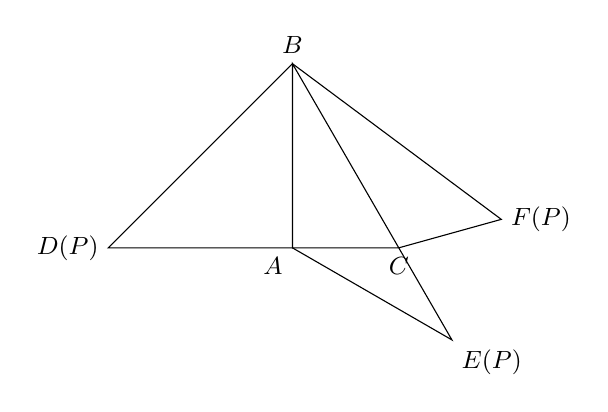
\begin{tikzpicture}[scale=1.35, font=\small]
  \coordinate (A) at (0,0);
  \coordinate (B) at (0,1.7320508);
  \coordinate (C) at (1,0);
  \coordinate (D) at (-1.7320508,0);
  \coordinate (E) at (1.5,-0.8660254);   % √3·(cos(-30°),sin(-30°))
  \coordinate (F) at (1.9641,0.2679);    % 由 FC=EC=1、FB=DB=√6 解出
  \draw (A) -- (B) -- (C) -- cycle;      % 中心三角形（折痕）
  \draw (B) -- (D) -- (A);               % △DAB
  \draw (A) -- (E) -- (C);               % △AEC
  \draw (C) -- (F) -- (B);               % △CFB
  \node[below left]  at (A) {$A$};
  \node[above]       at (B) {$B$};
  \node[below]       at (C) {$C$};
  \node[left]        at (D) {$D(P)$};
  \node[below right] at (E) {$E(P)$};
  \node[right]       at (F) {$F(P)$};
\end{tikzpicture}
